

%% AAPT Physics Bowl Exams Questions
%%----------------------------------------


% This section has 36 problems


%% PhysicsBowl 2015
%%----------------------------------------
\element{aapt}{ %% Bowl-A2
\begin{question}{bowl-2015-q05}
    An object initially is moving upward while in free fall.
    Which one of the following choices best represents the direction of the object's acceleration during its flight?
    \begin{center}
    \begin{tabu}{cX[c]X[c]X[c]}
        \toprule
        \makebox[1.5em][c]{\textnumero}
            & Object moving upward
            & Object at peak of motion
            & Object moving downward \\
        \bottomrule
    \end{tabu}
    \end{center}
    \begin{choices}
        \wrongchoice{\begin{tabu}{X[c]X[c]X[c]} Upward & Zero & Downward \\ \end{tabu}}
        \wrongchoice{\begin{tabu}{X[c]X[c]X[c]} Downward & Zero & Downward \\ \end{tabu}}
        \wrongchoice{\begin{tabu}{X[c]X[c]X[c]} Upward & Downward & Downward \\ \end{tabu}}
        \wrongchoice{\begin{tabu}{X[c]X[c]X[c]} Downward & Zero & Upward \\ \end{tabu}}
      \correctchoice{\begin{tabu}{X[c]X[c]X[c]} Downward & Downward & Downward \\ \end{tabu}}
    \end{choices}
\end{question}
}

\element{aapt}{ %% Bowl-A2
\begin{question}{bowl-2015-q07}
    An object moves clockwise with constant speed around the vertical circle shown.
    \begin{center}
    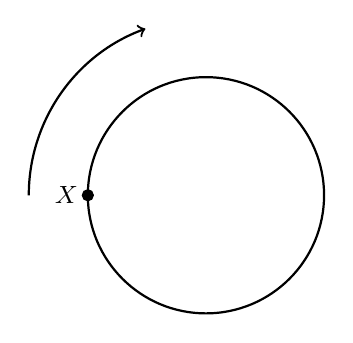
\begin{tikzpicture}[font=\small]
        \draw[thick] (0,0) circle (1.5cm);
        \draw[fill] (-1.5,0) circle (2pt) node[anchor=east] {$X$};
        \draw[thick,->] (-2.25,0) arc (180:110:2.25cm);
    \end{tikzpicture}
    \end{center}
    Which arrow best indicates the direction of the object's
        instantaneous acceleration at the point labeled $X$?
    \begin{multicols}{3}
    \begin{choices}
        \AMCboxDimensions{down=-0.33cm}
        \correctchoice{
            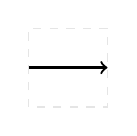
\begin{tikzpicture}
                \draw[white!90!black,dashed] (0,0) rectangle (1,1);
                \draw[thick,->] (0,0.5) -- (1,0.5);
            \end{tikzpicture}
        }
        \wrongchoice{
            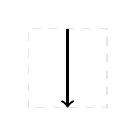
\begin{tikzpicture}
                \draw[white!90!black,dashed] (0,0) rectangle (1,1);
                \draw[thick,->] (0.5,1) -- (0.5,0);
            \end{tikzpicture}
        }
        \wrongchoice{
            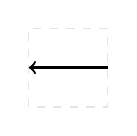
\begin{tikzpicture}
                \draw[white!90!black,dashed] (0,0) rectangle (1,1);
                \draw[thick,->] (1,0.5) -- (0,0.5);
            \end{tikzpicture}
        }
        \wrongchoice{
            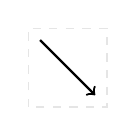
\begin{tikzpicture}
                \draw[white!90!black,dashed] (0,0) rectangle (1,1);
                \draw[thick,->] (0.15,0.85) -- (0.85,0.15);
            \end{tikzpicture}
        }
        \wrongchoice{
            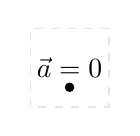
\begin{tikzpicture}
                \draw[white!90!black,dashed] (0,0) rectangle (1,1);
                \draw[fill] (0.5,0.25) circle (1.5pt)
                    node[anchor=south] {$\vec{a}=0$};
            \end{tikzpicture}
        }
        %\wrongchoice{There is no acceleration}
    \end{choices}
    \end{multicols}
\end{question}
}

\element{aapt}{ %% Bowl-A2
\begin{question}{bowl-2015-q14}
    A particle has a position, $x$, as a function of time, $t$,
    given as $x(t) = -\num{15} -\num{25}t + \num{10}t^2$.
    Which one of the following choices represents
        the magnitude of the particle's acceleration?
    %All quantities are expressed in base SI units.
    \begin{multicols}{3}
    \begin{choices}
        \wrongchoice{\SI{5}{\meter\per\second\squared}}
        \wrongchoice{\SI{10}{\meter\per\second\squared}}
        \wrongchoice{\SI{15}{\meter\per\second\squared}}
      \correctchoice{\SI{20}{\meter\per\second\squared}}
        \wrongchoice{\SI{40}{\meter\per\second\squared}}
        %% NOTE: added for symmetry
        \wrongchoice{\SI{25}{\meter\per\second\squared}}
    \end{choices}
    \end{multicols}
\end{question}
}

\element{aapt}{ %% Bowl-A2
\begin{question}{bowl-2015-q21}
    An object is launched from the ground at an angle of \ang{60}
        above the horizontal with a speed of \SI{20.0}{\second}.
    What is the magnitude of the average velocity of the object
        from just after launch until it reaches its highest vertical position during flight?
    \begin{multicols}{2}
    \begin{choices}
        \wrongchoice{\SI{13.7}{\meter\per\second}}
      \correctchoice{\SI{13.2}{\meter\per\second}}
        \wrongchoice{\SI{10.0}{\meter\per\second}}
        \wrongchoice{\SI{9.3}{\meter\per\second}}
        \wrongchoice{\SI{8.7}{\meter\per\second}}
    \end{choices}
    \end{multicols}
\end{question}
}

\element{aapt}{ %% Bowl-A2
\begin{question}{bowl-2015-q23}
    A car moves with constant speed around a horseshoe-shaped
        path as shown with the arrows in the figure.
    \begin{center}
    \begin{tikzpicture}
    \begin{scope}[very thick,decoration={markings,mark=at position 0.5 with {\arrow{latex}}}] 
        %% Inner bottom to inner upper
        \draw[postaction={decorate}] (2,-1.25) arc(270:450:0.125) -- (0,-1);
        \draw[postaction={decorate}] (0,-1) arc (270:90:1cm);
        \draw[postaction={decorate}] (0,+1) -- (2,1); %arc(270:450:0.125);
        %% outer upper to  outer bottom
        \draw[postaction={decorate}] (2,1) arc(270:450:0.125) -- (0,1.25) arc(90:180:1.25);
        \draw[postaction={decorate}] (-1.25,0) arc(180:270:1.25cm) -- (2,-1.25);
        %% X and W Labels
        \draw[fill] (1,-1.25) circle (2pt) node[anchor=north] {$W$};
        \draw[fill] (-1.25,0) circle (2pt) node[anchor=east] {$X$};
    \end{scope}
    \end{tikzpicture}
    \end{center}
    Which one of the following choices best describes the direction
        of the average acceleration of the car in traveling from $W$ to $X$?
    \begin{multicols}{3}
    \begin{choices}
        \AMCboxDimensions{down=-0.33cm}
        \correctchoice{
            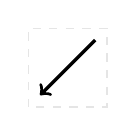
\begin{tikzpicture}
                \draw[white!90!black,dashed] (0,0) rectangle (1,1);
                \draw[very thick,->] (0.85,0.85) -- (0.15,0.15);
            \end{tikzpicture}
        }
        \wrongchoice{
            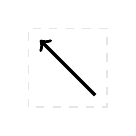
\begin{tikzpicture}
                \draw[white!90!black,dashed] (0,0) rectangle (1,1);
                \draw[very thick,->] (0.85,0.15) -- (0.15,0.85);
            \end{tikzpicture}
        }
        \wrongchoice{
            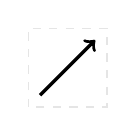
\begin{tikzpicture}
                \draw[white!90!black,dashed] (0,0) rectangle (1,1);
                \draw[very thick,->] (0.15,0.15) -- (0.85,0.85);
            \end{tikzpicture}
        }
        \wrongchoice{
            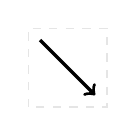
\begin{tikzpicture}
                \draw[white!90!black,dashed] (0,0) rectangle (1,1);
                \draw[very thick,->] (0.15,0.85) -- (0.85,0.15);
            \end{tikzpicture}
        }
        \wrongchoice{
            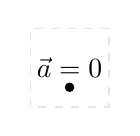
\begin{tikzpicture}
                \draw[white!90!black,dashed] (0,0) rectangle (1,1);
                \draw[fill] (0.5,0.25) circle (1.5pt) node[anchor=south] {$\vec{a}=0$};
            \end{tikzpicture}
        }
        %\wrongchoice{There is no average acceleration}
    \end{choices}
    \end{multicols}
\end{question}
}

\element{aapt}{ %% Bowl-A2
\begin{question}{bowl-2015-q36}
    Rain falls vertically at \SI{12.0}{\meter\per\second} with respect to a stationary observer.
    A car is moving at an angle of \ang{40} below the horizontal with respect to the observer.
    A passenger sitting in the car notes that the rain makes an angle of \ang{29.0} with the vertical.
    What is the car's speed with respect to the observer?
    \begin{multicols}{2}
    \begin{choices}
        \wrongchoice{\SI{2.29}{\meter\per\second}}
      \correctchoice{\SI{5.39}{\meter\per\second}}
        \wrongchoice{\SI{9.03}{\meter\per\second}}
        \wrongchoice{\SI{11.8}{\meter\per\second}}
        \wrongchoice{\SI{16.2}{\meter\per\second}}
    \end{choices}
    \end{multicols}
\end{question}
}


%% PhysicsBowl 2014
%%----------------------------------------
\element{aapt}{ %% Bowl-A2
\begin{question}{bowl-2014-q03}
    An object is dropped into free fall.
    Through how many meters does the object fall during the first \SI{3.00}{\second} of flight?
    \begin{multicols}{3}
    \begin{choices}
        \wrongchoice{\SI{10.0}{\meter}.}
        \wrongchoice{\SI{15.0}{\meter}.}
        \wrongchoice{\SI{30.0}{\meter}.}
      \correctchoice{\SI{45.0}{\meter}.}
        \wrongchoice{\SI{90.0}{\meter}.}
    \end{choices}
    \end{multicols}
\end{question}
}

\element{aapt}{ %% Bowl-A2
\begin{question}{bowl-2014-q40}
    A small \SI{1.35}{\kilo\gram} mass is launched from the top of a cliff at an angle of \ang{15.9} above the horizontal.
    \begin{center}
    \begin{tikzpicture}
        %% Surface
        \draw[thick] (0,3) -- (1,3) -- (1,0) -- (3,0);
        %% Top Arrow
        \coordinate (A) at (1,3.1);
        \draw[fill] (A) circle (1pt);
        \draw[thick,->] (A) -- ++ (15.9:1cm);
        \draw[dashed] (A) -- ++ (0:1cm) node [anchor=south west] {\ang{15.9}};
        %% Bottom Arrow
        \coordinate (B) at (3,0);
        \draw[fill] (B) circle (1pt);
        \draw[thick,->] (B) -- ++ (-34.4:1cm);
        \draw[dashed] (B) -- ++ (0:1cm) node[anchor=north west] {\ang{34.4}};
    \end{tikzpicture}
    \end{center}
    When the mass reaches the ground \SI{4.33}{\second} later,
        its velocity is directed at \ang{34.4} below the horizontal.
    What is the speed of the mass when it reaches the ground?
    Ignore air resistance.
    \begin{multicols}{3}
    \begin{choices}
        \wrongchoice{\SI{60.7}{\meter\per\second}}
      \correctchoice{\SI{54.1}{\meter\per\second}}
        \wrongchoice{\SI{46.4}{\meter\per\second}}
        \wrongchoice{\SI{43.3}{\meter\per\second}}
        \wrongchoice{\SI{38.8}{\meter\per\second}}
    \end{choices}
    \end{multicols}
\end{question}
}


%% PhysicsBowl 2013
%%----------------------------------------
\element{aapt}{ %% Bowl-A2
\begin{question}{bowl-2013-q02}
    A small object is released from rest and reaches the ground in a time of \SI{2.50}{\second}.
    With what speed does the object reach the ground?
    Neglect air resistance.
    \begin{multicols}{3}
    \begin{choices}
        \wrongchoice{\SI{31.3}{\meter\per\second}}
      \correctchoice{\SI{25.0}{\meter\per\second}}
        \wrongchoice{\SI{12.5}{\meter\per\second}}
        \wrongchoice{\SI{10.0}{\meter\per\second}}
        \wrongchoice{\SI{2.50}{\meter\per\second}}
    \end{choices}
    \end{multicols}
\end{question}
}

\element{aapt}{ %% Bowl-A2
\begin{question}{bowl-2013-q03}
    A small object is released from rest and reaches the ground in a time of \SI{2.50}{\second}.
    From what height above the ground was the object being released?
    Neglect air resistance.
    \begin{multicols}{3}
    \begin{choices}
        \wrongchoice{\SI{6.25}{\meter}}
        \wrongchoice{\SI{12.5}{\meter}}
        \wrongchoice{\SI{25.0}{\meter}}
      \correctchoice{\SI{31.3}{\meter}}
        \wrongchoice{\SI{62.5}{\meter}}
    \end{choices}
    \end{multicols}
\end{question}
}

\element{aapt}{ %% Bowl-A2
\begin{question}{bowl-2013-q10}
    An object is thrown straight upward.
    The object remains in free fall until it returns to its initial launch point.
    Which one of the following graphs could represent the velocity of the object as a function of time during the flight?
    \begin{multicols}{2}
    \begin{choices}
        \AMCboxDimensions{down=-2.0em}
        \wrongchoice{
            \begin{tikzpicture}
                \begin{axis}[
                    axis y line=left,
                    axis x line=middle,
                    axis line style={->},
                    xlabel={time},
                    xtick=\empty,
                    x label style={anchor=north east},
                    ylabel={velocity},
                    ytick=\empty,
                    xmin=0,xmax=11,
                    ymin=-5.5,ymax=5.5,
                    width=0.95\columnwidth,
                    very thin,
                ]
                \addplot[line width=1pt,domain=0:5]{5-x};
                \addplot[line width=1pt,domain=5:10]{(x-5)};
                \end{axis}
            \end{tikzpicture}
        }
        \wrongchoice{
            \begin{tikzpicture}
                \begin{axis}[
                    axis y line=left,
                    axis x line=middle,
                    axis line style={->},
                    xlabel={time},
                    xtick=\empty,
                    x label style={anchor=south east},
                    ylabel={velocity},
                    ytick=\empty,
                    xmin=0,xmax=11,
                    ymin=-5.5,ymax=5.5,
                    width=0.95\columnwidth,
                    very thin,
                ]
                \addplot[line width=1pt,domain=0:5]{-5+x};
                \addplot[line width=1pt,domain=5:10]{(5-x)};
                \end{axis}
            \end{tikzpicture}
        }
        \wrongchoice{
            \begin{tikzpicture}
                \begin{axis}[
                    axis y line=left,
                    axis x line=middle,
                    axis line style={->},
                    xlabel={time},
                    xtick=\empty,
                    x label style={anchor=north east},
                    ylabel={velocity},
                    ytick=\empty,
                    xmin=0,xmax=11,
                    ymin=-5.5,ymax=5.5,
                    width=0.95\columnwidth,
                    very thin,
                ]
                \addplot[line width=1pt,domain=0:10]{0.2*(x-5)*(x-5)};
                \end{axis}
            \end{tikzpicture}
        }
        \wrongchoice{
            \begin{tikzpicture}
                \begin{axis}[
                    axis y line=left,
                    axis x line=middle,
                    axis line style={->},
                    xlabel={time},
                    xtick=\empty,
                    x label style={anchor=south east},
                    ylabel={velocity},
                    ytick=\empty,
                    xmin=0,xmax=11,
                    ymin=-5.5,ymax=5.5,
                    width=0.95\columnwidth,
                    very thin,
                ]
                \addplot[line width=1pt,domain=0:10]{-0.2*(x-5)*(x-5)};
                \end{axis}
            \end{tikzpicture}
        }
        \correctchoice{
            \begin{tikzpicture}
                \begin{axis}[
                    axis y line=left,
                    axis x line=middle,
                    axis line style={->},
                    xlabel={time},
                    xtick=\empty,
                    x label style={anchor=south east},
                    ylabel={velocity},
                    ytick=\empty,
                    xmin=0,xmax=11,
                    ymin=-5.5,ymax=5.5,
                    width=0.95\columnwidth,
                    very thin,
                ]
                \addplot[line width=1pt,domain=0:10]{5-x};
                \end{axis}
            \end{tikzpicture}
        }
        %% NOTE:
    \end{choices}
    \end{multicols}
\end{question}
}

\element{aapt}{ %% Bowl-A2
\begin{question}{bowl-2013-q14}
    A small box is thrown at an angle of \ang{30.0} above the horizontal ground with a speed of \SI{20.0}{\meter\per\second}.
    To what maximum height above the launch point does the ball rise during its motion?
    Ignore air resistance.
    \begin{multicols}{3}
    \begin{choices}
        \wrongchoice{\SI{2.5}{\meter}}
      \correctchoice{\SI{5.0}{\meter}}
        \wrongchoice{\SI{10.0}{\meter}}
        \wrongchoice{\SI{15.0}{\meter}}
        \wrongchoice{\SI{20.0}{\meter}}
    \end{choices}
    \end{multicols}
\end{question}
}

\element{aapt}{ %% Bowl-A2
\begin{questionmult}{bowl-2013-q18}
    Which of the following choices correctly identifies a situations for which there is a non-zero acceleration?
    \begin{choices}
      \correctchoice{A point object moves in a straight line with increasing speed.}
      \correctchoice{A point object moves in a circular path with constant speed.}
      \correctchoice{A point object moves in a circular path with decreasing speed.}
    \end{choices}
\end{questionmult}
}

\element{aapt}{ %% Bowl-A2
\begin{question}{bowl-2013-q33}
    At the top of a high cliff, a small rock is dropped from rest.
    A ball is launched straight downward with an initial speed of \SI{36.0}{\meter\per\second} at a time \SI{2.10}{\second} after the rock was dropped.
    When the ball has fallen \SI{28.0}{\meter} further than the initially dropped rock,
        what is the speed of the ball relative to the rock?
    \begin{multicols}{2}
    \begin{choices}
      \correctchoice{\SI{15.0}{\meter\per\second}}
        \wrongchoice{\SI{16.0}{\meter\per\second}}
        \wrongchoice{\SI{20.0}{\meter\per\second}}
        \wrongchoice{\SI{21.0}{\meter\per\second}}
        \wrongchoice{\SI{36.0}{\meter\per\second}}
    \end{choices}
    \end{multicols}
\end{question}
}


%% PhysicsBowl 2012
%%----------------------------------------
\element{aapt}{ %% Bowl-A2
\begin{question}{bowl-2012-q26}
    An object is thrown horizontally with speed
        \SI{10.0}{\meter\per\second} from a height
        $H$ above the ground.
    The object reaches the ground with a speed of
        \SI{20.0}{\meter\per\second}.
    Which one of the following choices best represents
        the time of the object's flight to the ground?
    Ignore air resistance.
    \begin{multicols}{3}
    \begin{choices}
        \wrongchoice{\SI{1.00}{\second}}
        \wrongchoice{\SI{1.22}{\second}}
        \wrongchoice{\SI{1.41}{\second}}
        \wrongchoice{\SI{1.50}{\second}}
      \correctchoice{\SI{1.73}{\second}}
    \end{choices}
    \end{multicols}
\end{question}
}


%% PhysicsBowl 2009
%%----------------------------------------

%% NOTE: bowl-2009-q09

\element{aapt}{ %% Bowl-A2
\begin{question}{bowl-2009-q20}
    A projectile launched from the ground landed a horizontal
        distance of \SI{120.0}{\meter} from its launch point.
    The projectile was in the air for a time of \SI{4.00}{\second}.
    If the projectile landed at the same vertical position from
        which it was launched, what was the launch speed of the
        projectile?
    Ignore air resistance.
    \begin{multicols}{3}
    \begin{choices}
        \wrongchoice{\SI{22.4}{\meter\per\second}}
        \wrongchoice{\SI{30.0}{\meter\per\second}}
      \correctchoice{\SI{36.1}{\meter\per\second}}
        \wrongchoice{\SI{42.4}{\meter\per\second}}
        \wrongchoice{\SI{50.0}{\meter\per\second}}
    \end{choices}
    \end{multicols}
\end{question}
}


%% PhysicsBowl 2008
%%----------------------------------------
\newcommand{\BowlTwentyZeroEightQFourteen}{
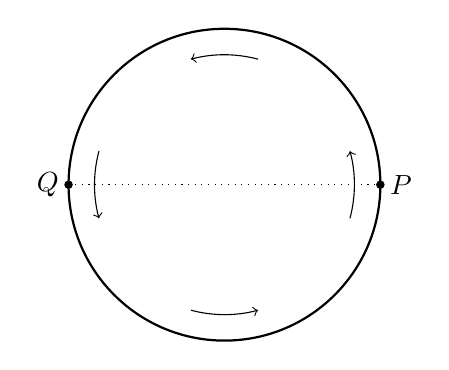
\begin{tikzpicture}[scale=0.66]
    \draw[thick] (0,0) circle (3cm);
    \draw[fill] (+3,0) circle (2pt) node[anchor=west] {$P$};
    \draw[fill] (-3,0) circle (2pt) node[anchor=east] {$Q$};
    \draw[dotted] (-3,0) -- (+3,0);
    \foreach \a/\b in {-15/15,75/105,165/195,255/285} {
        \draw[->] (\a:2.5cm) arc (\a:\b:2.5cm);
    }
\end{tikzpicture}
}

\element{aapt}{ %% Bowl-A2
\begin{question}{bowl-2008-q14}
    A particle continuously moves in a circular path at constant speed in a counter-clockwise direction.
    Consider a time interval during which the particle moves along this circular path from point $P$ to point $Q$.
    Point $Q$ is exactly half-way around the circle from point $P$.
    \begin{center}
        \BowlTwentyZeroEightQFourteen
    \end{center}
    %% Start question
    What is the direction of the average velocity during this time interval?
    \begin{multicols}{2}
    \begin{choices}
        \AMCboxDimensions{down=-0.4cm}
        \wrongchoice{
            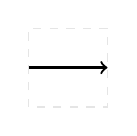
\begin{tikzpicture}
                \draw[dashed,draw=white!90!black] (0,0) rectangle (1,1);
                \draw[thick,->] (0,0.5) -- (1,0.5);
            \end{tikzpicture}
        }
        %% ANS is B
        \correctchoice{
            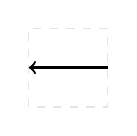
\begin{tikzpicture}
                \draw[dashed,draw=white!90!black] (0,0) rectangle (1,1);
                \draw[thick,->] (1,0.5) -- (0,0.5);
            \end{tikzpicture}
        }
        \wrongchoice{
            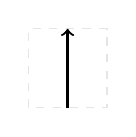
\begin{tikzpicture}
                \draw[dashed,draw=white!90!black] (0,0) rectangle (1,1);
                \draw[thick,->] (0.5,0) -- (0.5,1);
            \end{tikzpicture}
        }
        \wrongchoice{
            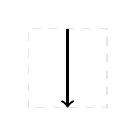
\begin{tikzpicture}
                \draw[dashed,draw=white!90!black] (0,0) rectangle (1,1);
                \draw[thick,->] (0.5,1) -- (0.5,0);
            \end{tikzpicture}
        }
        \wrongchoice{
            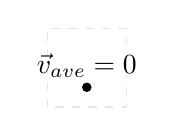
\begin{tikzpicture}
                \draw[dashed,draw=white!90!black] (0,0) rectangle (1,1);
                \draw[fill] (0.5,0.25) circle (1.5pt) node[anchor=south] {$\vec{v}_{ave}=0$};
            \end{tikzpicture}
        }
    \end{choices}
    \end{multicols}
\end{question}
}

\element{aapt}{ %% Bowl-A2
\begin{question}{bowl-2008-q15}
    A particle continuously moves in a circular path at constant speed in a counter-clockwise direction.
    Consider a time interval during which the particle moves along this circular path from point $P$ to point $Q$.
    Point $Q$ is exactly half-way around the circle from point $P$.
    \begin{center}
        \BowlTwentyZeroEightQFourteen
    \end{center}
    %% Start question
    What is the direction of the average acceleration during this time interval?
    \begin{multicols}{3}
    \begin{choices}
        \AMCboxDimensions{down=-0.4cm}
        \wrongchoice{
            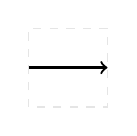
\begin{tikzpicture}
                \draw[dashed,draw=white!90!black] (0,0) rectangle (1,1);
                \draw[thick,->] (0,0.5) -- (1,0.5);
            \end{tikzpicture}
        }
        \wrongchoice{
            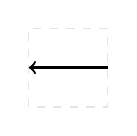
\begin{tikzpicture}
                \draw[dashed,draw=white!90!black] (0,0) rectangle (1,1);
                \draw[thick,->] (1,0.5) -- (0,0.5);
            \end{tikzpicture}
        }
        \wrongchoice{
            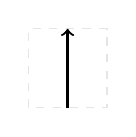
\begin{tikzpicture}
                \draw[dashed,draw=white!90!black] (0,0) rectangle (1,1);
                \draw[thick,->] (0.5,0) -- (0.5,1);
            \end{tikzpicture}
        }
        %% ANS is D
        \correctchoice{
            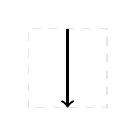
\begin{tikzpicture}
                \draw[dashed,draw=white!90!black] (0,0) rectangle (1,1);
                \draw[thick,->] (0.5,1) -- (0.5,0);
            \end{tikzpicture}
        }
        \wrongchoice{
            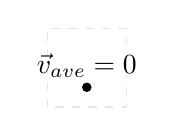
\begin{tikzpicture}
                \draw[dashed,draw=white!90!black] (0,0) rectangle (1,1);
                \draw[fill] (0.5,0.25) circle (1.5pt) node[anchor=south] {$\vec{v}_{ave}=0$};
            \end{tikzpicture}
        }
    \end{choices}
    \end{multicols}
\end{question}
}


%% PhysicsBowl 2006
%%----------------------------------------
\element{aapt}{ %% Bowl-A2
\begin{question}{bowl-2006-q04}
    An arrow is shot from a bow at an angle of \ang{40} from the
        horizontal at a speed of \SI{24.0}{\meter\per\second}.
    Ignoring air resistance,
        what is the arrow's maximum height above its launch point?
    \begin{multicols}{3}
    \begin{choices}
        \wrongchoice{\SI{5.9}{\meter}}
      \correctchoice{\SI{11.9}{\meter}}
        \wrongchoice{\SI{16.9}{\meter}}
        \wrongchoice{\SI{23.8}{\meter}}
        \wrongchoice{\SI{28.8}{\meter}}
    \end{choices}
    \end{multicols}
\end{question}
}

\element{aapt}{ %% Bowl-A2
\begin{question}{bowl-2006-q13}
    A rock is dropped from the top of a tall tower.
    Half a second later another rock,
        twice as massive as the first,
        is dropped.
    Ignoring air resistance,
    \begin{choices}
      \correctchoice{the distance between the rocks increases while both are falling.}
        \wrongchoice{the acceleration is greater for the more massive rock.}
        \wrongchoice{the speed of both rocks is constant while they fall.}
        \wrongchoice{they strike the ground more than half a second apart.}
        \wrongchoice{they strike the ground with the same kinetic energy.}
    \end{choices}
\end{question}
}


\element{aapt}{ %% Bowl-A2
\begin{question}{bowl-2006-q22}
    During an interval of time, a tennis ball is moved so that the
        angle between the velocity and the acceleration of the ball
        is kept at a constant \ang{120}.
    Which statement is true about the tennis ball during this interval of time?
    \begin{choices}
        \wrongchoice{Its speed increases and it is changing its direction of travel.}
      \correctchoice{Its speed decreases and it is changing its direction of travel.}
        \wrongchoice{Its speed remains constant, but it is changing its direction of travel.}
        \wrongchoice{Its speed remains constant and it is not changing its direction of travel.}
        \wrongchoice{Its speed decreases and it is not changing its direction of travel.}
    \end{choices}
\end{question}
}


%% PhysicsBowl 2005
%%----------------------------------------
\element{aapt}{ %% Bowl-A2
\begin{question}{bowl-2005-q02}
    A pebble is dropped from a high vertical cliff.
    The collision of the pebble with the ground below is seen
       \SI{1.50}{\second} after the pebble is dropped.
    With what speed did the pebble hit the ground?
    Ignore air resistance.
    \begin{multicols}{3}
    \begin{choices}
        \wrongchoice{\SI{10}{\meter\per\second}}
      \correctchoice{\SI{15}{\meter\per\second}}
        \wrongchoice{\SI{48.6}{\meter\per\second}}
        \wrongchoice{\SI{100.4}{\meter\per\second}}
        \wrongchoice{\SI{343}{\meter\per\second}}
    \end{choices}
    \end{multicols}
\end{question}
}

\element{aapt}{ %% Bowl-A2
\begin{question}{bowl-2005-q35}
    An arrow is shot horizontally toward a target \SI{20}{\meter} away.
    In traveling the first \SI{5}{\meter} horizontally,
        the arrow falls \SI{0.2}{\meter}.
    In traveling the next \SI{5}{\meter} horizontally it will fall an additional
    \begin{multicols}{3}
    \begin{choices}
      \correctchoice{\SI{0.6}{\meter}}
        \wrongchoice{\SI{0.4}{\meter}}
        \wrongchoice{\SI{0.3}{\meter}}
        \wrongchoice{\SI{0.2}{\meter}}
        \wrongchoice{\SI{0.1}{\meter}}
    \end{choices}
    \end{multicols}
\end{question}
}


%% PhysicsBowl 2000
%%----------------------------------------
\element{aapt}{ %% Bowl-A2
\begin{question}{bowl-2000-q37}
    %The next TWO questions will refer to the following information.
    During a recent winter storm,
        bales of hay had to be dropped from an airplane to a herd of cattle below.
    Assume the airplane flew horizontally at an altitude of \SI{180}{\meter}
        with a constant velocity of \SI{50}{\meter\per\second} and dropped
        one bail of hay every \SI{2}{\second}.
    It is reasonable to assume that air resistance will be negligible for this situation.
    As the bales are falling through the air,
        what will happen to their distance of separation?
    \begin{choices}
      \correctchoice{the distance of separation will increase}
        \wrongchoice{the distance of separation will decrease}
        \wrongchoice{the distance of separation will remain constant}
        \wrongchoice{the distance of separation will depend on the mass of the bales}
        \wrongchoice{none of the provided are always true}
    \end{choices}
\end{question}
}

\element{aapt}{ %% Bowl-A2
\begin{question}{bowl-2000-q38}
    %The next TWO questions will refer to the following information.
    During a recent winter storm,
        bales of hay had to be dropped from an airplane to a herd of cattle below.
    Assume the airplane flew horizontally at an altitude of \SI{180}{\meter}
        with a constant velocity of \SI{50}{\meter\per\second} and dropped
        one bail of hay every \SI{2}{\second}.
    It is reasonable to assume that air resistance will be negligible for this situation.
    About how far apart from each other will the bales land on the ground?
    \begin{multicols}{3}
    \begin{choices}
        \wrongchoice{\SI{9000}{\meter}}
        \wrongchoice{\SI{300}{\meter}}
        \wrongchoice{\SI{180}{\meter}}
      \correctchoice{\SI{100}{\meter}}
        \wrongchoice{\SI{50}{\meter}}
    \end{choices}
    \end{multicols}
\end{question}
}

\element{aapt}{ %% Bowl-A2
\begin{question}{bowl-2000-q39}
    If a boat can travel with a speed of $v$ in still water,
        which of the following trips will take the least amount of time.
    \begin{choices}
      \correctchoice{traveling a distance of $2d$ in still water}
        \wrongchoice{traveling a distance of $2d$ across (perpendicular to) the current in a stream}
        \wrongchoice{traveling a distance $d$ downstream and returning a distance $d$ upstream}
        \wrongchoice{traveling a distance $d$ upstream and returning a distance $d$ downstream}
        \wrongchoice{all of the provided will take equal times}
    \end{choices}
\end{question}
}


%% PhysicsBowl 2000
%%----------------------------------------
\element{aapt}{ %% Bowl-A2
\begin{question}{bowl-1999-q06}
    An airplane with air speed \SI{120}{\kilo\meter\per\hour}
        is heading due north in a wind blowing due east at
        \SI{50}{\kilo\meter\per\hour}.
    What is the ground speed of the plane?
    \begin{multicols}{2}
    \begin{choices}
        \wrongchoice{\SI{60}{\kilo\meter\per\hour}}
        \wrongchoice{\SI{120}{\kilo\meter\per\hour}}
      \correctchoice{\SI{130}{\kilo\meter\per\hour}}
        \wrongchoice{\SI{140}{\kilo\meter\per\hour}}
        \wrongchoice{None of these}
    \end{choices}
    \end{multicols}
\end{question}
}

\element{aapt}{ %% Bowl-A2
\begin{question}{bowl-1999-q07}
    In the absence of air resistance, if an object were
        to fall freely near the surface of the Moon.
    \begin{choices}
        \wrongchoice{its velocity could never exceed \SI{10}{\meter\per\second}.}
        \wrongchoice{its acceleration would gradually decrease until the object moves with a terminal velocity.}
      \correctchoice{the acceleration is constant.}
        \wrongchoice{it will fall with a constant speed.}
        \wrongchoice{the acceleration is zero.}
    \end{choices}
\end{question}
}

\element{aapt}{ %% Bowl-A2
\begin{question}{bowl-1999-q09}
    If air resistance can be neglected, what happens to the
        horizontal velocity component of a basketball as it
        is thrown to the basket from the free-throw line?
    \begin{choices}
        \wrongchoice{increases}
        \wrongchoice{decreases}
        \wrongchoice{decreases until the ball reaches the top then increases as the ball comes down}
        \wrongchoice{increases until the ball reaches the top then decreases as the ball comes down}
      \correctchoice{remains constant}
    \end{choices}
\end{question}
}


%% PhysicsBowl 1998
%%----------------------------------------
\element{aapt}{ %% Bowl-A2
\begin{question}{bowl-1998-q13}
    When a falling object moves with terminal velocity, it:
    \begin{choices}
        \wrongchoice{has zero velocity.}
      \correctchoice{has zero acceleration.}
        \wrongchoice{has an upward acceleration.}
        \wrongchoice{is no longer subject to air resistance.}
        \wrongchoice{has an acceleration of approximately \SI{10}{\meter\per\second\squared}.}
    \end{choices}
\end{question}
}

\element{aapt}{ %% Bowl-A2
\begin{question}{bowl-1998-q40}
    Coin I is thrown upward from the top of a \SI{100}{\meter} tower with speed of \SI{15}{\meter\per\second}.
    Coin II is dropped (zero initial speed) from the top of the tower \SI{2.0}{\second} later.
    Assume $g$ is \SI{10}{\meter\per\second\squared}.
    How far below the top of the tower does coin I pass coin II?
    \begin{multicols}{3}
    \begin{choices}
        \wrongchoice{\SI{1.6}{\meter}}
        \wrongchoice{\SI{16}{\meter}}
      \correctchoice{\SI{20}{\meter}}
        \wrongchoice{\SI{80}{\meter}}
        \wrongchoice{\SI{96}{\meter}}
    \end{choices}
    \end{multicols}
\end{question}
}


%% PhysicsBowl 1997
%%----------------------------------------
\element{aapt}{ %% Bowl-A2
\begin{question}{bowl-1997-q09}
    At a certain time,
        an object in free fall has velocity \SI{4.0}{\meter\per\second} in the upward direction.
    What is the approximate velocity of the object one second later?
    \begin{multicols}{2}
    \begin{choices}
        \wrongchoice{\SI{14}{\meter\per\second} up}
        \wrongchoice{\SI{10}{\meter\per\second} up}
        \wrongchoice{\SI{4.0}{\meter\per\second} up}
      \correctchoice{\SI{6.0}{\meter\per\second} down}
        \wrongchoice{\SI{10}{\meter\per\second} down}
    \end{choices}
    \end{multicols}
\end{question}
}

\element{aapt}{ %% Bowl-A2
\begin{question}{bowl-1997-q40}
    A boat is traveling at \SI{6.0}{\kilo\meter\per\hour} \ang{30} W of N with respect to a river.
    The river is flowing at \SI{3.0}{\kilo\meter\per\hour} from W to E.
    As observed from shore, the boat is traveling:
    \begin{multicols}{2}
    \begin{choices}
        \wrongchoice{\ang{45} E of N}
        \wrongchoice{\ang{30} E of N}
      \correctchoice{due N}
        \wrongchoice{\ang{30} W of N}
        \wrongchoice{\ang{45} W of N}
    \end{choices}
    \end{multicols}
\end{question}
}


%% PhysicsBowl 1996
%%----------------------------------------
\element{aapt}{ %% Bowl-A2
\begin{question}{bowl-1996-q08}
    A ball is rolled off the edge of a horizontal table.
    The ball has an initial speed $v_0$ and lands on the floor some distance from the base of the table.
    Which of the following statements concerning the fall of the ball is \emph{false}?
    \begin{choices}
        \wrongchoice{The time of flight depends on the height of the table.}
        \wrongchoice{One of the components of the final speed will be $v_0$.}
        \wrongchoice{The ball will accelerate.}
      \correctchoice{The ball will have a longer flight time if $v_0$ is increased.}
        \wrongchoice{The ball will fall because of the force due to gravity.}
    \end{choices}
\end{question}
}


%% PhysicsBowl 1995
%%----------------------------------------
\element{aapt}{ %% Bowl-A2
\begin{question}{bowl-1995-q19}
    A baseball is thrown horizontally from a cliff.
    At the same instant, a bowling ball is dropped from the same height.
    Assuming air resistance can be ignored,
        which of the following statements is correct?
    \begin{choices}
        \wrongchoice{The bowling ball hits the ground first.}
      \correctchoice{Both the baseball and the bowling ball hit the ground at the same time.}
        \wrongchoice{The baseball has the greater acceleration just before it hits the ground.}
        \wrongchoice{The bowling ball has the greater velocity just before it hits the ground.}
        \wrongchoice{The bowling ball has the greater acceleration just before it hits the ground.}
    \end{choices}
\end{question}
}

\element{aapt}{ %% Bowl-A2
\begin{question}{bowl-1995-q27}
    A rocket near the surface of the earth is accelerating vertically upward at \SI{10}{\meter\per\second\squared}.
    The rocket releases an instrument package.
    Immediately after release the acceleration of the instrument package is:
    \begin{multicols}{2}
    \begin{choices}
        \wrongchoice{\SI{20}{\meter\per\second\squared} up}
        \wrongchoice{\SI{10}{\meter\per\second\squared} up}
        \wrongchoice{\SI{0}{\meter\per\second\squared}}
      \correctchoice{\SI{10}{\meter\per\second\squared} down}
        \wrongchoice{\SI{20}{\meter\per\second\squared} down}
    \end{choices}
    \end{multicols}
\end{question}
}


%% PhysicsBowl 1995
%%----------------------------------------
\element{aapt}{ %% Bowl-A2
\begin{question}{bowl-1994-q03}
    A ball is thrown off a high cliff with no horizontal velocity.
    It lands \SI{6.0}{\second} later with a velocity of \SI{40.0}{\meter\per\second}.
    What was the initial velocity of the ball?
    \begin{multicols}{2}
    \begin{choices}
        \wrongchoice{\SI{100}{\meter\per\second} up}
      \correctchoice{\SI{20}{\meter\per\second} up}
        \wrongchoice{\SI{0}{\meter\per\second}}
        \wrongchoice{\SI{20}{\meter\per\second} down}
        \wrongchoice{\SI{100}{\meter\per\second} down}
    \end{choices}
    \end{multicols}
\end{question}
}


%% PhysicsBowl 1994
%%----------------------------------------
\element{aapt}{ %% Bowl-A2
\begin{question}{bowl-1994-q14}
    An arrow is aimed horizontally,
        directly at the center of a target \SI{20}{\meter} away.
    The arrow hits \SI{0.050}{\meter} below the center of the target.
    Neglecting air resistance, what was the initial speed of the arrow?
    \begin{multicols}{3}
    \begin{choices}
        \wrongchoice{\SI{20}{\meter\per\second}}
        \wrongchoice{\SI{40}{\meter\per\second}}
        \wrongchoice{\SI{100}{\meter\per\second}}
      \correctchoice{\SI{200}{\meter\per\second}}
        \wrongchoice{\SI{400}{\meter\per\second}}
    \end{choices}
    \end{multicols}
\end{question}
}


\endinput



